%FOR PDFLATEX USE ONLY
\documentclass[a4paper,12pt]{article}

\usepackage{amssymb,amsmath} %math symbols

\usepackage[margin=2cm]{geometry} %paper geometry

\usepackage[utf8]{inputenc} %allows unicode (including russian) source file
\usepackage[russian]{babel} %docment in russian-style
\usepackage[utf8]{inputenc}
%\usepackage[unicode]{hyperref} %links inside of the text
\usepackage[pdftex]{graphicx} %includegraphics pictures
\usepackage{cmlgc} %bold text

\usepackage{array} %arrays

%\usepackage{wrapfig}
%\usepackage{array}
%\usepackage{lipsum}
%\usepackage{esvect}
%\usepackage{hyperref}

\usepackage{subfig}
%\usepackage{calc}
%\usepackage{pgfplots,tikz,circuitikz}
%\usepackage{tkz-euclide}
\usepackage{booktabs}
\usepackage{multirow}

\usepackage{wrapfig}

\begin{document}

\begin{center}
  \LARGE{Работа 4.7.3}\\[0.2cm]
  \LARGE{Изучение поляризованного света}\\[0.2cm]
  \large{Балдин Виктор}\\[0.2cm]
\end{center}

\textbf{Цель работы}: ознакомление с методами получения и анализа поляризованного света.


\textbf{В работе используются}: оптическая скамья с осветителем; зеленый светофильтр; два поляроида; черное зеркало; полированная эбонитовая пластинка; стопа стеклянных пластинок; слюдяные пластинки разной толщины; пластинки в $1/4$ и $1/2$ длины волны; пластинка в одну длины полны для зеленого цвета (пластинка чувствительного оттенка).
\section*{Теория}

При помощи специальных приспособлений (поляризаторов), естественный свет может быть превращен в линейно поляризованный (или, как иногда говорят, в плоскополяризованный). В линейно поляризованной световой волне пара векторов \textbf{E} и \textbf{H} не изменяет с течением времени своей ориентации. Плоскость \textbf{E, S} называется в этом случае \textit{плоскостью колебаний}. \par
Наиболее общим типом поляризации является \textit{эллиптическая поляризация}. В эллиптически поляризованной световой волне конец вектора
\textbf{E} (в данной точке пространства) описывает некоторый эллипс. Линейно
поляризованный свет можно рассматривать как частный случай эллиптически поляризованного света, когда эллипс поляризации вырождается в отрезок прямой линии; другим частным случаем является круговая
поляризация (эллипс поляризации является окружностью). \par
Для получения линейно поляризованного света применяются специальные оптические приспособления — поляризаторы. Направление колебаний электрического вектора в волне, прошедшей через поляризатор, называется
разрешенным направлением поляризатора.
Всякий поляризатор может быть использован для исследования поляризованного света, т. е. в качестве анализатора. Интенсивность I линейно поляризованного света после прохождения через анализатор зависит от угла, образованного плоскостью колебаний с разрешенным направлением анализатора:
\begin{equation}
  I = I_0 \cos^2\alpha.
\end{equation}
Соотношение (1) носит название \textit{закона Малюса}. \par
. Отраженный от диэлектрика свет всегда частично поляризован. Степень поляризации света, отраженного от диэлектрической пластинки в воздух, зависит от показателя преломления диэлектрика $n$ и от угла падения $\alpha$. Как следует из формул Френеля, полная поляризация отраженного света достигается
при падении под \textit{углом Брюстера}, который определяется соотношением
\begin{equation}
 \tg \alpha = n.
\end{equation}

В этом случае плоскость колебаний электрического вектора в отраженном свете перпендикулярна плоскости падения. Для увеличения степени поляризации преломлённого
света используют стопу стеклянных пластинок, расположенных под углом Брюстера к падающему свету.

% \section*{Результаты и обработка}
% \subsection*{Определение разрешенных направлений поляроидов}
% Разместим на оптической скамье осветитель $S$, поляроид $P$ и черное зеркало. Методом последовательных приближений найдем такое расположение поляроида и зеркала, что интенсивность отраженного света минимальна.

% \begin{center}
% 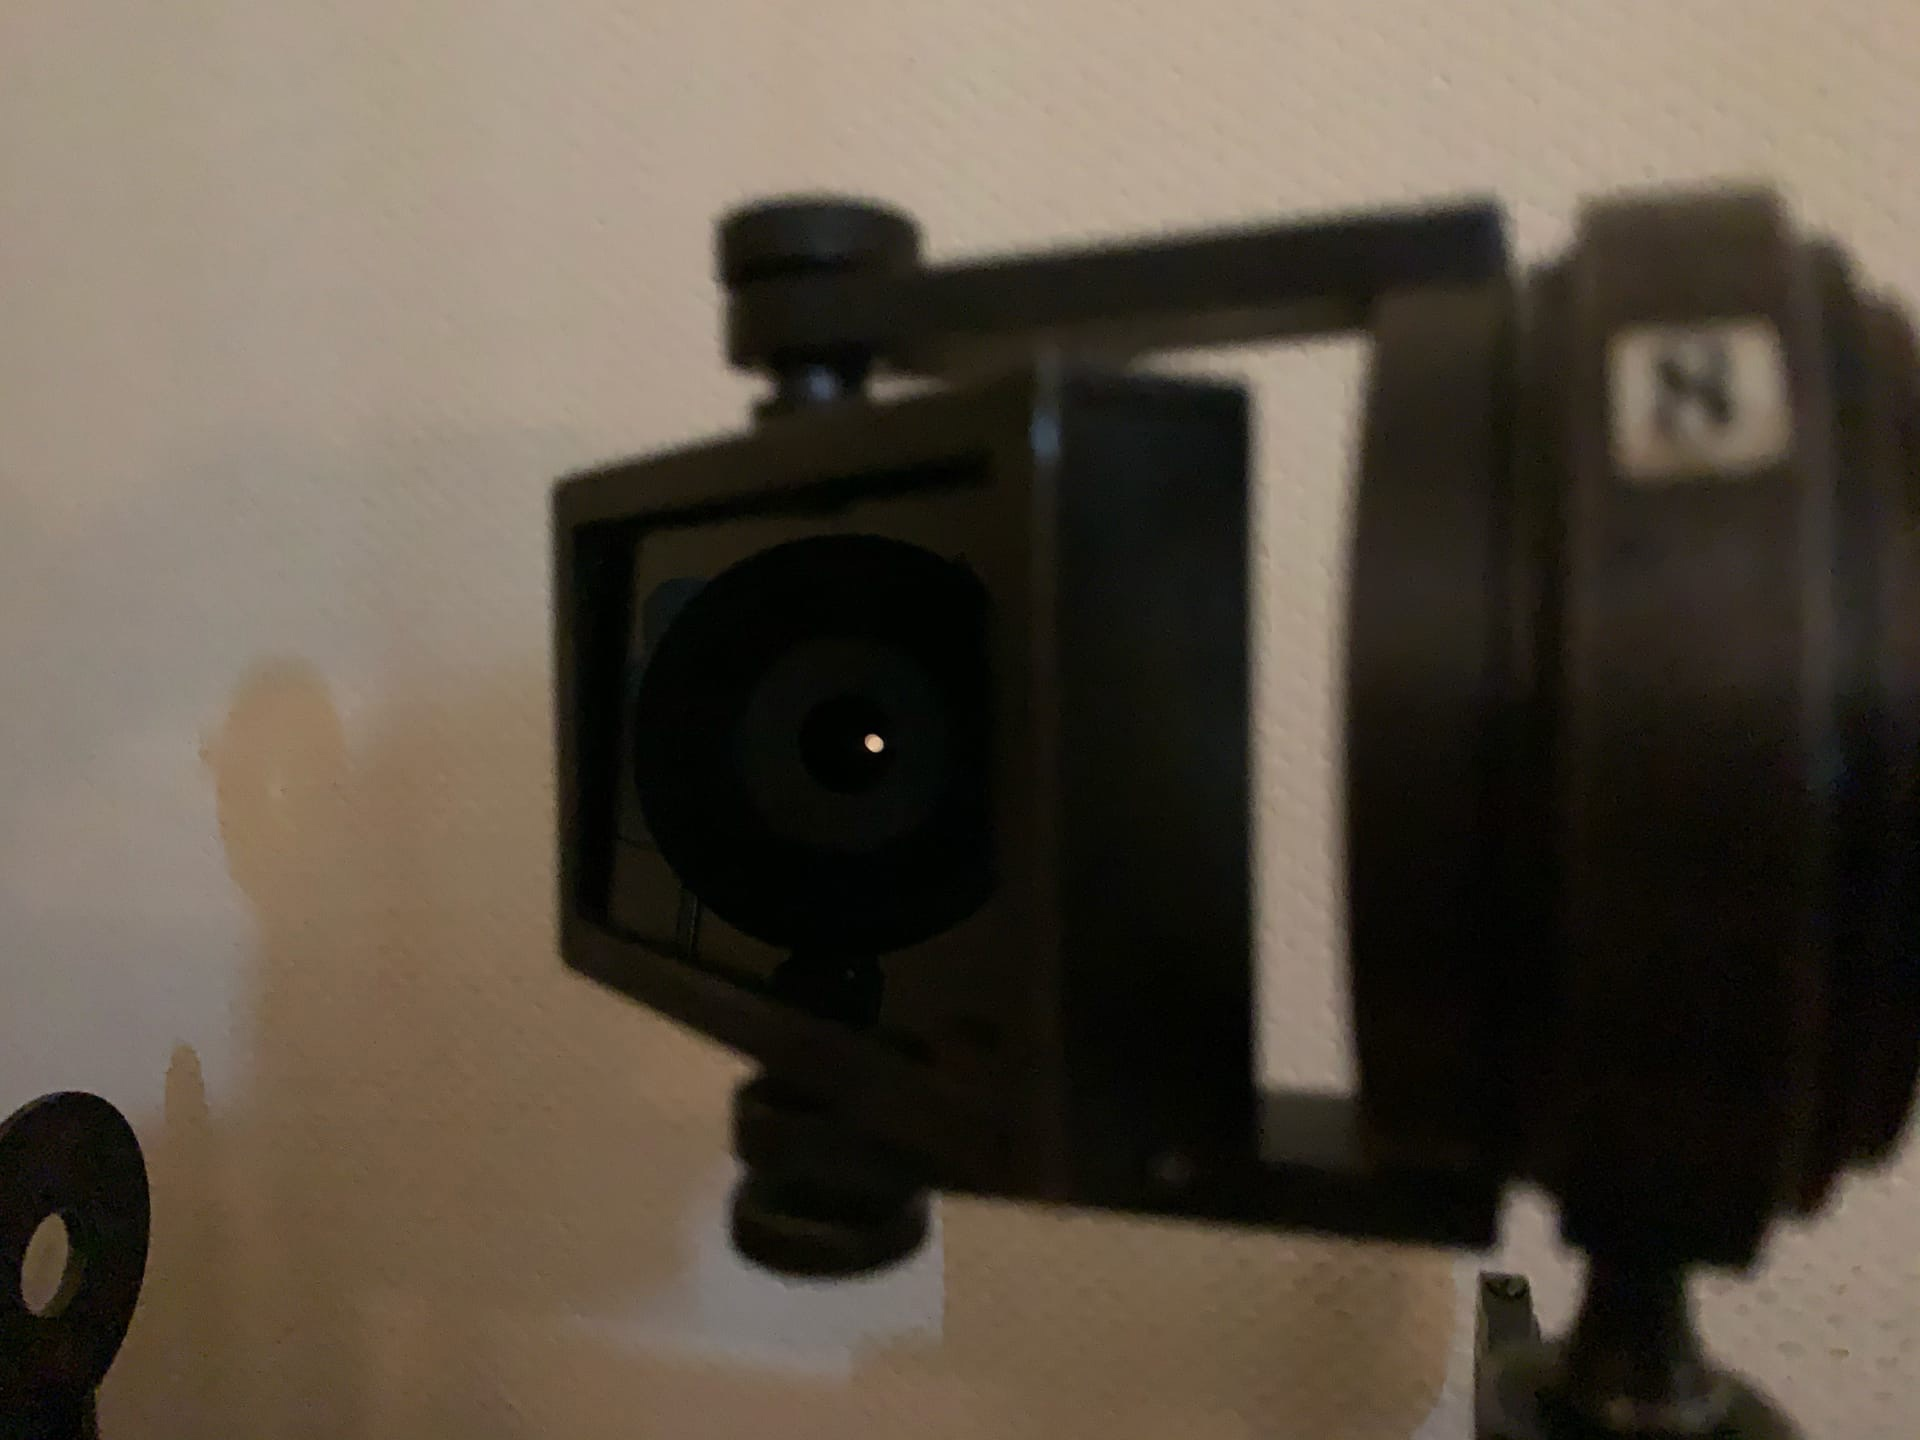
\includegraphics[width=0.80\textwidth]{1.png}\\
% изображение источника в зеркале
% \end{center}

% \begin{center}
% 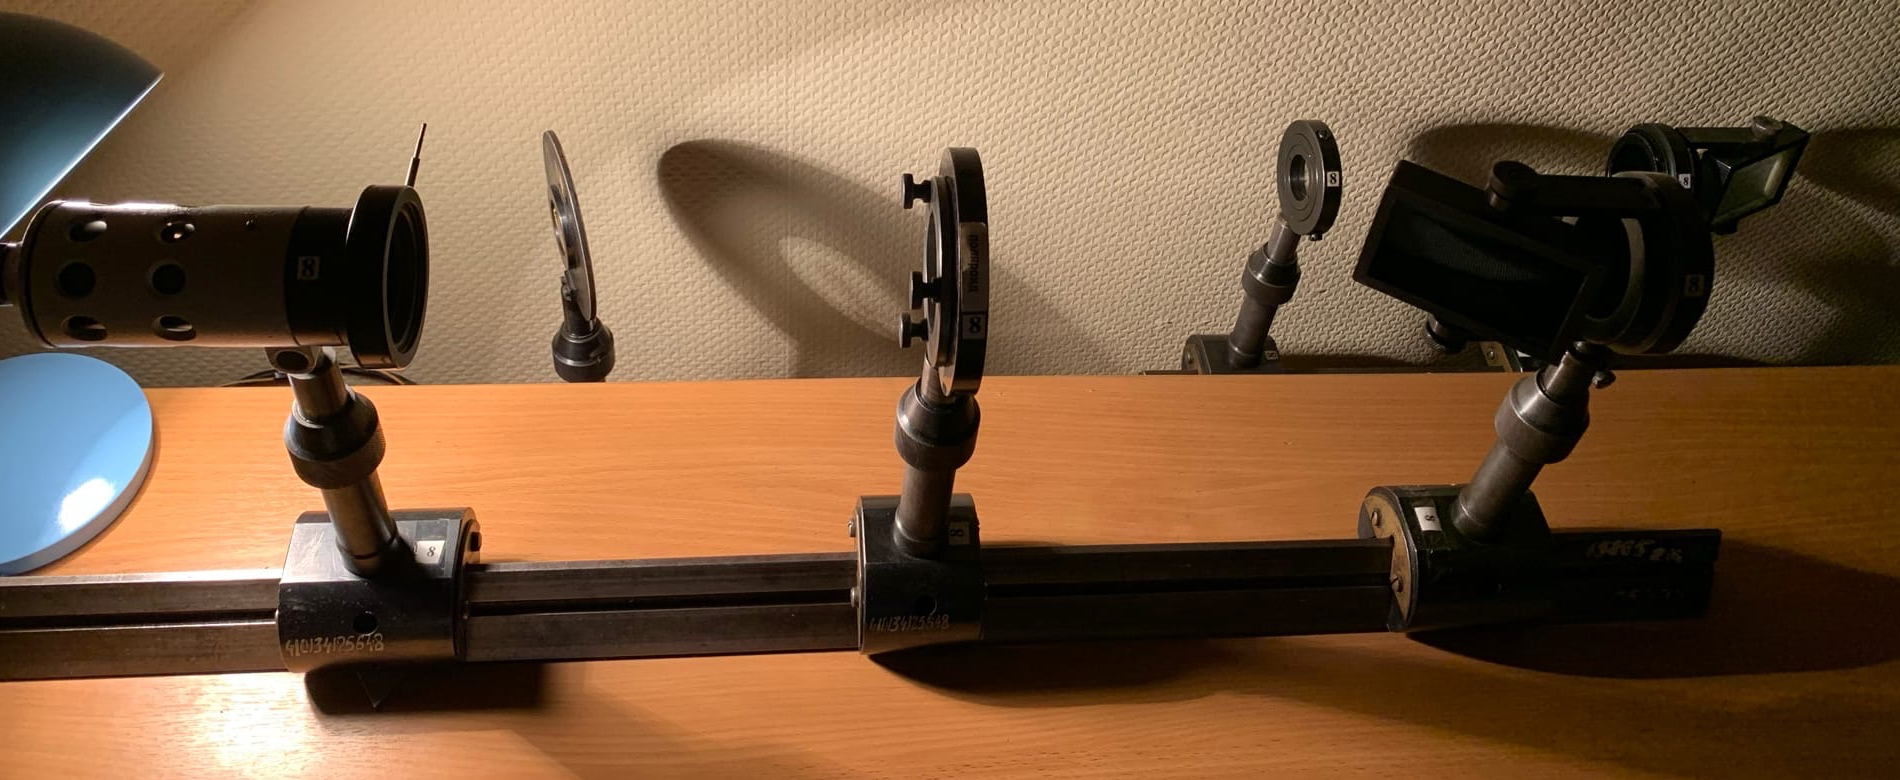
\includegraphics[width=0.80\textwidth]{2.png}\\
% установка
% \end{center}

% Разрешенное направление второго поляроида можно определить, скрестив поляроиды.

% \subsection*{Определение угла Брюстера для эбонита}
% Найдем показатель преломления эбонита. Для этого посмотрим на свет источника $S$, отраженный от эбонитовой пластинки. Меняя угол поворота пластинки, добьемся того, чтобы интенсивность света после прохождения через поляризатор была минимальна. Это будет означать, что свет падает под углом Брюстера $\alpha = arctan(n)$

% \begin{center}
% 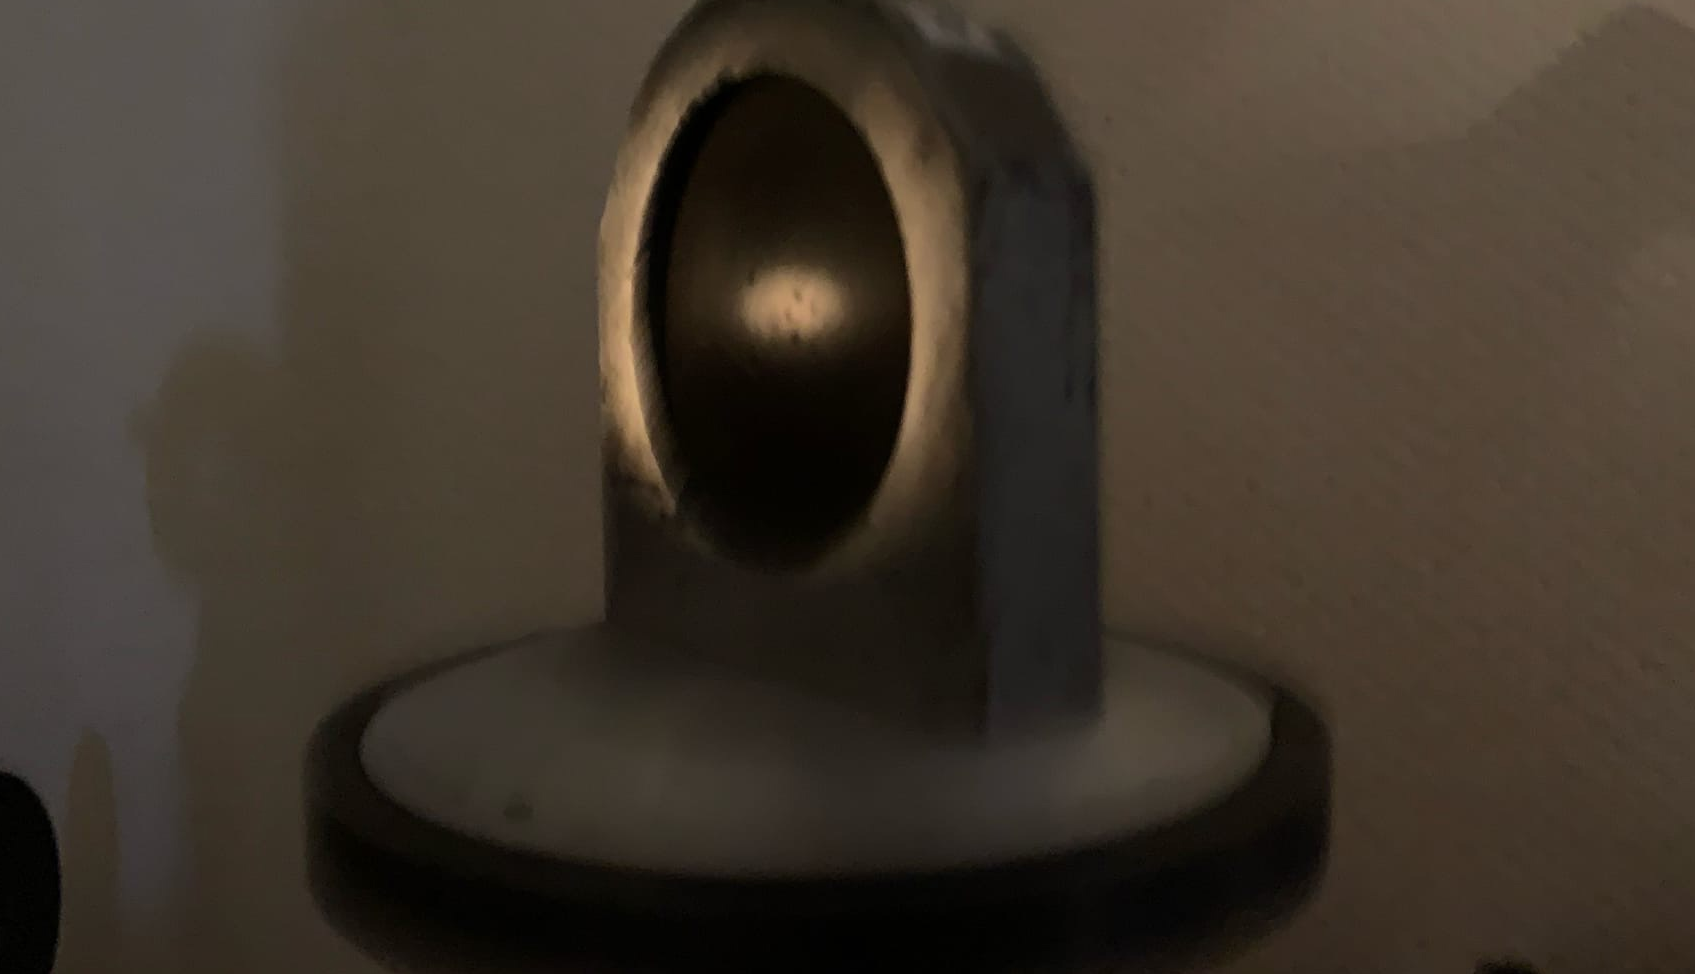
\includegraphics[width=0.80\textwidth]{3.png}\\
% свет, отраженный от пластинки
% \end{center}

% В результате получается значение

% \[n=\tan((60 \pm 5)^\circ)=1.4\pm0.3.\]

% \subsection*{Исследование стопы}
% Происследуем стопу. Поставим стопу стеклянных пластинок вместо эбонитового зеркала и добьемся того, чтобы свет падал на стопу под углом Брюстера.

% \begin{center}
% 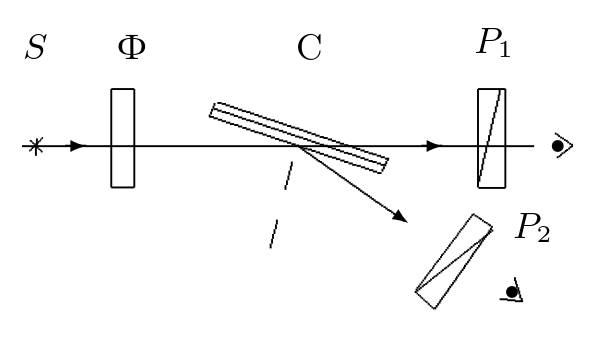
\includegraphics[width=0.50\textwidth]{4.png}\\
% Исследование стопы
% \end{center}

% Происследуем свет, отраженный и прошедший через стопу с помощью поляризаторов. Получим, что свет, отраженный от стопы поляризован вертикально, а прошедший через стопу --- горизонтально.

% \subsection*{Определение главных плоскостей двоякопреломляющих пластин}

% Поставим клисталлическую пластинку между скрещенными поляроидами $P_1$ и $P_2$. И происследуем интенсивность света, прошедшего через систему от угла поворота пластинки. В момент, когда главные оси совпадают с плоскостями поляроидов, интенсивность минимальная. Это происходит 4 раза за поворот.



% \begin{center}
% 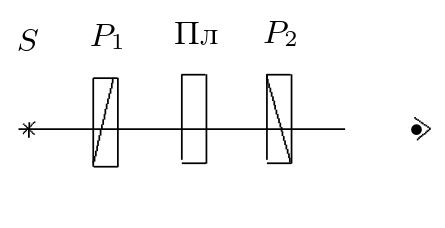
\includegraphics[width=0.50\textwidth]{5.png}\\
% Определение главных направлений в пластинках
% \end{center}

% \subsection*{Выделение пластин $\lambda/2$ и $\lambda/4$}
% Если добавить к схеме выше зеленый фильтр и повернуть главные направления в пластинке на угол $45^\circ$, то можно будет определить тип пластинки по поляризованности света, выходящего из неё. Происследуем зависимость интенсивности света, проходящего через установку, от угла поворота последнего поляризатора $P_2$. Если пластинка $\lambda/2$, свет поляризуем линейно и минимумы интенсивности наблюдаются 2 раза за оборот. Если пластинка $\lambda/4$, то минимумы интенсивности не наблюдаются из-за того, что свет имеет круговую поляризацию.

% \subsection*{Эллиптически поляризованная волна}
% Пронаблюдаем эллиптически поляризованную волну. Для этого установим плоскость первого поляризатора под углом $10-20^\circ$ к горизонту. После него установим пластинку $\lambda/4$ с осями перпендикулярно и прараллельно земле.
% При повороте второго поляроида можно пронаблюдать эллиптическую поляризованность -- интенсивность заметно меняется, но не уходит в 0.

% Не сложно аналитически понять, что происходит. Для этого рассмотрим луч после первого поляризатора
% \[E_{1x} = \cos\alpha E_0 \sin(\omega t),\,E_{1y} = \sin\alpha E_0 \sin(\omega t) E_0,\]
% и после пластинки (если по $y$ замедление на $\lambda / 4$)
% \[E_{1x} = \cos\alpha E_0 \sin(\omega t),\,E_{1y} = - \sin\alpha E_0 \cos(\omega t) E_0.\]

% \begin{center}
% 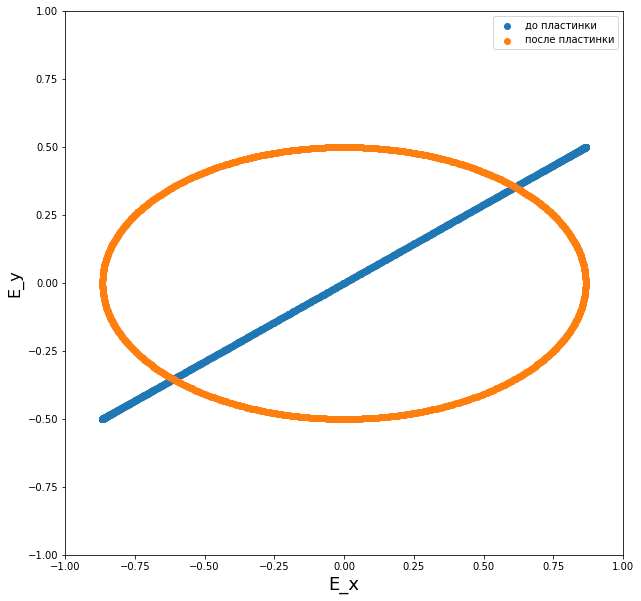
\includegraphics[width=0.50\textwidth]{7.png}\\
% Поляризация
% \end{center}

% \subsection*{Интерференция поляризованных лучей}
% Расположим между скрещенными поляроидами мозаичную слюдяную пластинку. Из описания лабораторной работы следует, что пластинка состоит из 4-х узких полосок слюды, лежащих по сторонам квадрата (две полоски $\lambda/4$, одна $\lambda/2$ и еще одна $3\lambda/3$).

% \begin{center}
% 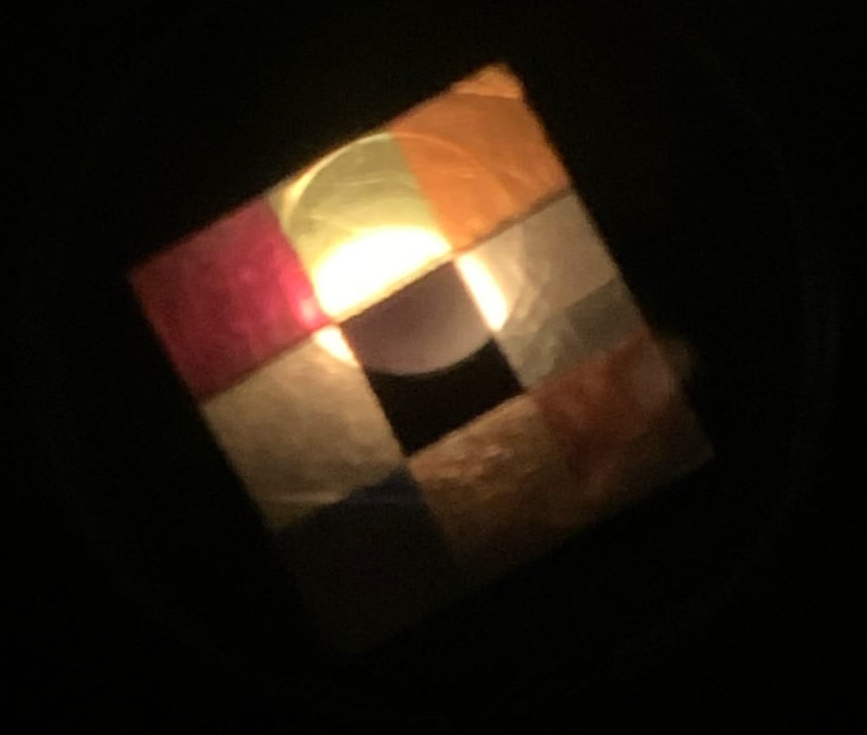
\includegraphics[width=0.50\textwidth]{6.png}\\
% мозаичная пластинка
% \end{center}

% Эксперимент показывает, что, если вращать пластинку, интенсивность света меняется с периодом в четверть оборота. Это происходит из-за того, что 4 раза за оборот оси пластинок совпадают с плоскостями поляризаторов.

% Также, если вращать поляризатор, меняется цвет пластинок 4 раза за оборот. Это происходит из-за того, что интенсивность не падает, поскольку поляризация круговая.

% \subsection*{Вывод}
% Мы провели несколько качественных эксперементов и узнали, как создавать и исследовать поляризованное излучение. Мы познакомились с линейной, круговой и эллиптической поляризацией.

\end{document}








% \lipsum[1-4]
% \begin{wrapfigure}{R}{5cm}
% \centering
% \includegraphics[width=0.20\textwidth]{rd.png}
% \caption{1}
% \end{wrapfigure}
% \lipsum[1-6]


% \begin{figure}[h]
% \begin{center}$
% \begin{array}{cccc}
% \includegraphics[width=0.20\textwidth]{rd.png}&
% \includegraphics[width=0.20\textwidth]{rd.png}&
% \includegraphics[width=0.20\textwidth]{rd.png}&
% \includegraphics[width=0.20\textwidth]{rd.png}\\
% (1) & (2) & (3) & (4)
% \end{array}$
% \end{center}
% \end{figure}
